\begin{figure}[H]
\center

\includegraphics[scale=1]{kibana.png}
\label{fig:kibana.png}
\end{figure}
\section{Qu'est ce que Kibana}
Kibana est un front-end à Elasticsearch permettant de présenter les données stockées dans ce dernier. 

C'est l'outil de visualisation officiel d'Elasticsearch, il est assez ergonomique 
et donc plutôt facile d'utilisation. Sa barre de recherche utilise la syntaxe 
\textit{search Lite} présentée précedemment dans le chapitre traitant d'Elasticsearch\footnote{voir p\pageref{subsec:elasticsearchlite}}.
Son utilisation pour réaliser des tableaux, dashboard (tableaux de bord) et autres
camemberts est assez aisée une fois les principes de bases assimilés.



\section{Installation de Kibana}
L'installation de Kibana est relativement simple, il suffit de télécharger l'application
compressée sur le site de \url{https://download.elastic.co/kibana/kibana/kibana-4.0.2-linux-x64.tar.gz}{elastic}.
On décompresse, on lance (\ipath{path/bin/kibana}), et c'est parti !
Évidemment, si on exécute Kibana d'une telle manière il est préférable de le lancer
depuis un quelconque multiplexeur de terminal (tmux,screen\ldots). 
Il est également facile de réaliser son propre service systemd.

\subsection{Paramétrage}
Afin de pouvoir se connecter à Elasticsearch il faut tout de même renseigner\\
\ipath{path/config/kibana.yml} notamment les paramètres : \emph{port} (par défaut 5601), \emph{host} (ip d'écoute)
et surtout \emph{elasticsearch\_url}.
Dans des circonstances normales c'est tout ce que vous aurez à paramétrer (hors 
SSL \ldots{}).

Il peut arriver dans de rares cas (lorsque Elasticsearch est saturé ou bien lors 
d'une requête particulièrement gourmande) que Kibana se ferme car Elasticsearch met
trop de temps à répondre. Il est dans ces cas là, fortement conseillé de 
redémarrer l'instance en question, d'étendre sa \emph{HEAP\_SIZE}, ou bien si possible, 
de rajouter de la RAM.

Il est possible de modifier le requestTimeout dans \ipath{path/src/lib/waitForEs.js}
C'est pour l'instant la seule façon de faire. D'après une issue github, la prochaine 
mouture de Kibana devrait intégrer ce paramètre dans son fichier de configuration.

\section{Utilisation de Kibana}
Dans cette partie nous allons faire une brève présentation (illustrée) de Kibana et
de son fonctionnement.

\subsection{Recherche}
\begin{figure}[H]
\center
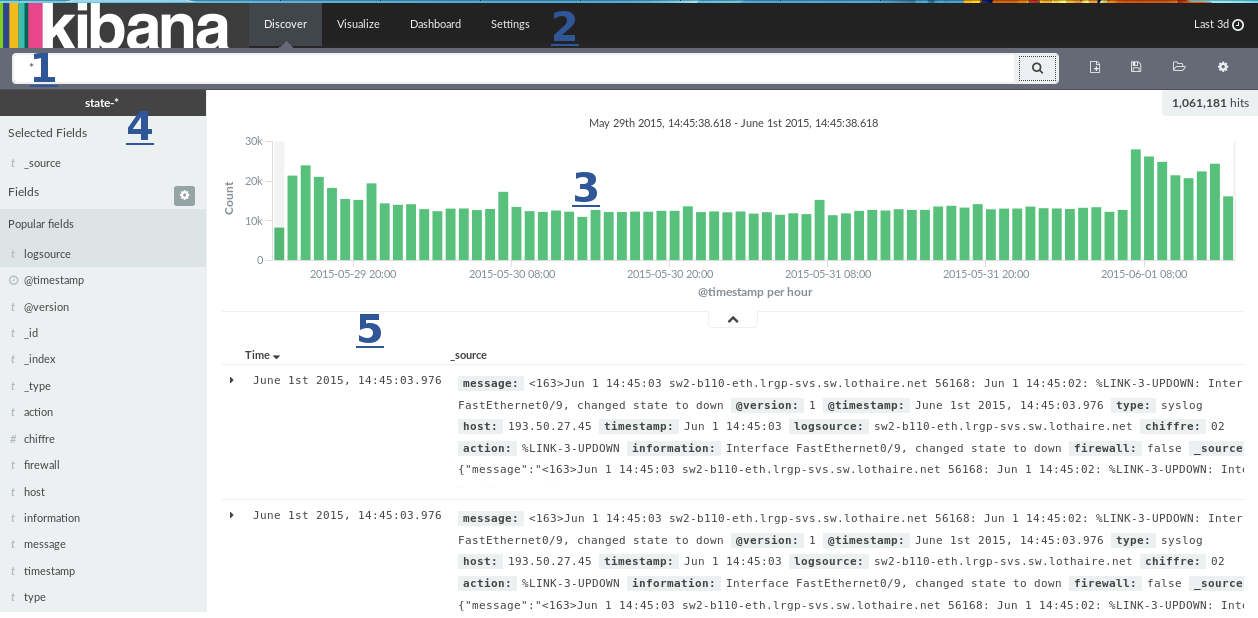
\includegraphics[width=1\textwidth]{kibanatuto/rap/1.png}
\label{fig:kibanatuto1}
\caption{Présentation générale de Kibana}
\end{figure}

Voici la page principale sur laquelle on arrive lorsque l'on se connecte à Kibana
depuis son navigateur.

\begin{enumerate}
    \item La barre de recherche \\(syntaxe SearchLite)
    \item Barre de sélection des \emph{modes} \\(Discover : Recherche, Visualize : Création 
    de Tableaux et autre représentations graphiques, Dashboard : Rassemblement de
    ces présentations, Settings : Paramétrage de certaines options)
    \item Tableau graphique des résultats de recherche
    \item Tableau des champs de l'index
    \item Tableaux des lignes correspondant à la recherche
\end{enumerate}


\begin{figure}[H]
\center
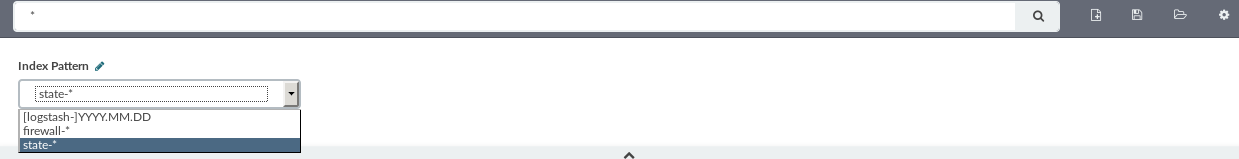
\includegraphics[width=1\textwidth]{kibanatuto/rap/2.png}
\label{fig:kibanatuto2}
\caption{Choisir son index pour une recherche}
\end{figure}
Pour effectuer une recherche, on doit préciser dans quels index. S'il est possible 
de réaliser une recherche dans plusieurs index à la fois,  mais ces deux index doivent 
disposer du même mapping (typiquement rangés par \ipath{nom-\{date\}}).
Pour choisir ses index il faut \emph{sélectionner la roue dentée à droite de la barre
de recherche}.


\begin{figure}[H]
\center
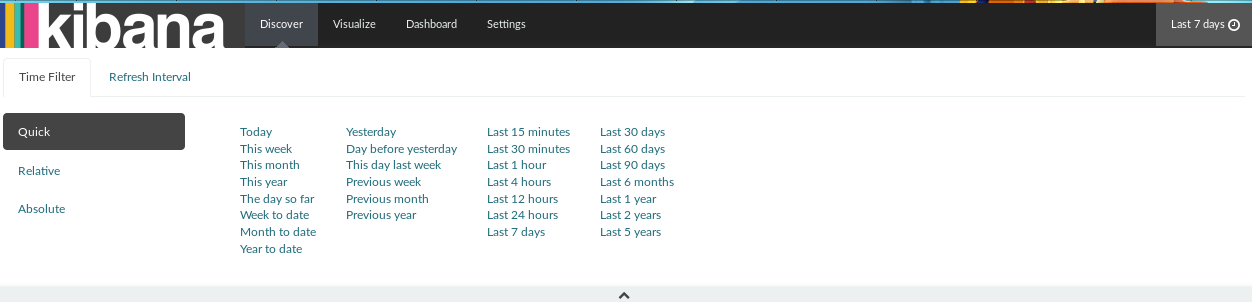
\includegraphics[width=1\textwidth]{kibanatuto/rap/3.png}
\label{fig:kibanatuto3}
\caption{Choisir son intervalle de temps}
\end{figure}
Lorsque l'on effectue une recherche avec Kibana il est possible de choisir de façon
très flexible son intervalle de temps (bouton de temps en haut à droite).
Il est tout d'abord possible de choisir les possibilités du menu rapide, affichées
dans l'image ci-dessus. Le choix est déjà assez exhaustif, mais il est également 
possible de se positionner relativement par à la date du jour. Par exemple rechercher 
parmi les 30 dernières secondes, ou bien les deux derniers mois (de la seconde à 
l'année). Il est également possible de choisir un intervalle de temps absolu, à 
la seconde près.

Enfin il est possible de rafraichir ces données en choisissant un intervalle allant
de 5 secondes à une journée (également désactivable).\\[2mm]
(Voir \textbf{tableau des champs} figure \ref{fig:kibanatuto4} p\pageref{fig:kibanatuto4})\\[2mm]

Le tableau des champs disponibles dans l'index est très pratique pour rendre plus 
lisibles les informations que l'on recherche ainsi que pour obtenir des statistiques 
rapides sur les occurrences des termes les plus communs.

Ce tableau contient tous les champs disponibles dans l'index. Il est possible de
faire de la ségrégation dans les résultats de nos recherches en incluant ou en   
excluant un ou plusieurs termes proposés {\footnotesize\textit{(on peut par exemple exclure le résultat 
le plus courant car on sait un switch défectueux, afin de se concentrer sur les autres
pannes pas encore détectées et donc plus pertinentes)}}. Il suffit pour cela d'appuyer
sur les loupes situées à droite des termes suggérés.


Il est également possible de choisir de ne montrer que \hyperref[fig:kibanatuto6]{la ou les parties que l'on 
estime pertinentes} dans le log (en appuyant sur le \hyperref[fig:kibanatuto5]{bouton 
add à droite} de chaque champ) et bien sûr de combiner les deux dernières "techniques".
\begin{figure}[H]
\begin{flushright}

\includegraphics[width=0.3\textwidth]{kibanatuto/rap/8.png}
\label{fig:kibanatuto5}
\end{flushright}%
\end{figure}

\begin{figure}[H]
\center
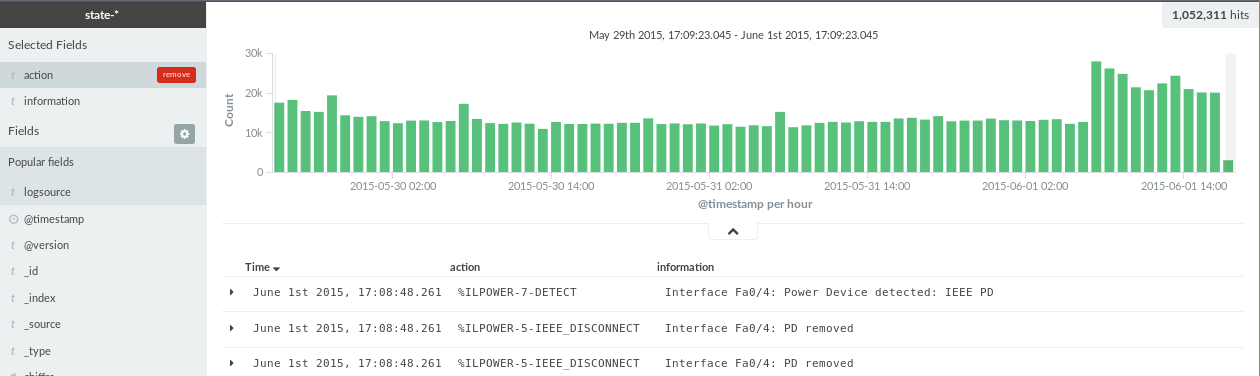
\includegraphics[width=1\textwidth]{kibanatuto/rap/9.png}
\label{fig:kibanatuto6}
\caption{Résultat}
\end{figure}

\subsection{Visualisation}
Nous allons maintenant parler de la visualisation des données, il s'agit là encore
seulement de donner un très bref aperçu des possibilités.\\[2mm]
(Voir \textbf{la page de garde des visualisations} \ref{fig:kibanatuto7} p\pageref{fig:kibanatuto7})\\[2mm]
Voilà les différents types de visualisations parmi lesquelles nous pouvons faire 
notre choix,  toutes ne conviennent pas. Le meilleur choix est affaire d'expérience.\\[2mm]
(Voir \textbf{le premier camembert} \ref{fig:kibanatuto8} p\pageref{fig:kibanatuto8})\\[2mm]
C'est un camembert très simple, réalisable en moins d'une minute. Il agrège les logs
sur une semaine en les classant par date d'émission, groupés par jour. 
Il est évidémment possible de faire des choses plus compliquées avec plus ou moins
données et de traitement.\\[2mm]
(Voir \textbf{les seconds camemberts} \ref{fig:kibanatuto9} p\pageref{fig:kibanatuto9})\\[2mm]
Chaque camembert représente une semaine. L'intérieur du camembert montre la répartition
par jour, l'anneau externe donne la répartition par tranche de 3 heures. Ces camemberts 
sont interactifs, on le verra dans la partie suivante sur les dashboards.


\subsection{Dashboard}
Présentons maintenant les dashboards. Sorte de tableaux virtuels, ils servent à rassembler
les informations. Ces informations ont normalement plus de sens une fois mises côte 
à côte ou permettent une analyse plus rapide d'une situation donnée.

La création de ces dashboards est également très simple, appuyer sur le \textit{plus}
en haut à droite.

Il suffit ensuite de choisir les visualisation et ou les recherches enregistrées 
que l'on souhaite voir affiché.\\[2mm]
(Voir l'image des \textbf{recherches et de la visualisation} \ref{fig:kibanatuto10} p\pageref{fig:kibanatuto10})\\[2mm]
Comme expliqué plus haut les visualisations ainsi que les tableaux sont interactifs.
Il est par exemple possible de façon assez intuitive d'effectuer une recherche limitée ségréguée.
Ici il suffit de cliquer sur le quartier désiré de la visualisation. Cela aura pour 
effet de faire apparaitre la barre verte (contextuelle) et de ne faire apparaitre 
dans le tableau de résultat à droite que les \gls{logs} correspondants. Ici les logs ayant
pour ip source 147.99.x.x affichés sur l'image ci-dessous.

\begin{figure}[H]
\center
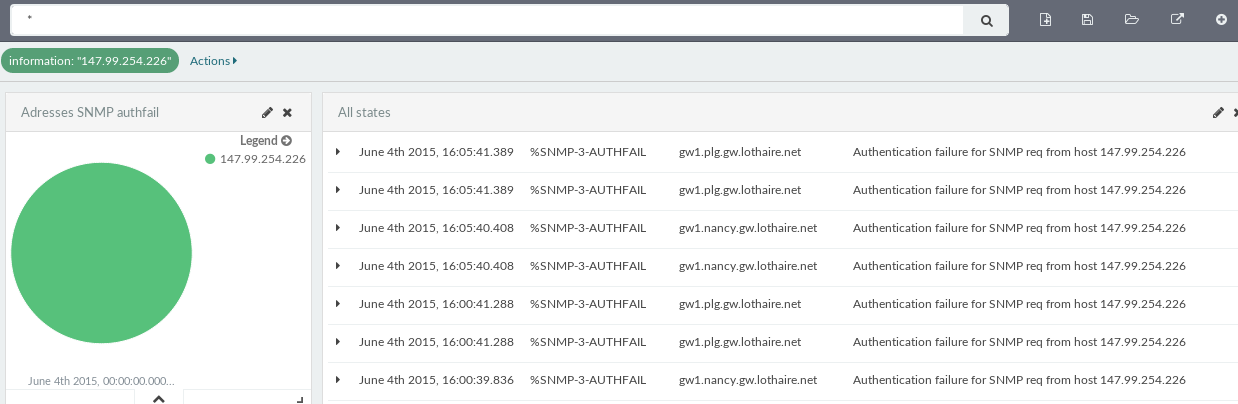
\includegraphics[width=1\textwidth]{kibanatuto/rap/18.png}
\label{fig:kibanatuto11}
\caption{Dashboard simple}
\end{figure}

Il est possible de partager facilement ces dashboard, via des liens avec 
iframes. On peut ainsi facilement les ajouter dans une page de monitoring par exemple.\\[2mm]
(Voir l'image d'un \textbf{Dashboard plus avancé} \ref{fig:kibanatuto12} p\pageref{fig:kibanatuto12})\\[2mm]
Partie non essentielle sur les \textbf{settings} p\pageref{subsec:settings}

\section{Conclusion}
Voici qui conclut la présentation des logiciels majeurs que nous avons
utilisés pour réaliser ce projet. Nous avons maintenant compris comment
centraliser et exporter les données, les ranger et maintenant les consulter.

%Kibana est sans doute le plus facile des trois  à prendre en main, et c'est heureux 
%car c'est celui avec lequel l'équipe interagira au quotidien.

Kibana facilite beaucoup l'exploration de données et permet, par l'intermédiaire 
des Dashboard,  de faciliter leur mise en corrélation. Ce logiciel peut facilement
être utilisé par tous avec très peu de formation.
